% ==============================================================================
% SECCIÓN 10: ANEXOS Y EVIDENCIAS ACADÉMICAS DEL PROYECTO
% ==============================================================================

\section{Anexos y Evidencias Académicas}

En esta sección se compilan las evidencias documentales, registros de auditoría de calidad, tableros de gestión ágil en Miro, estructuración de la EDT y registros fotográficos de las visitas técnicas realizadas por el equipo a las instalaciones de Comercial Machi's.

\subsection{Anexo A: Gestión de Proyecto, EDT y Tableros Ágiles en Miro}

El proyecto fue planificado y controlado mediante la Estructura de Desglose de Trabajo (EDT) y tableros Kanban en la plataforma colaborativa Miro:

\begin{figure}[H]
\centering
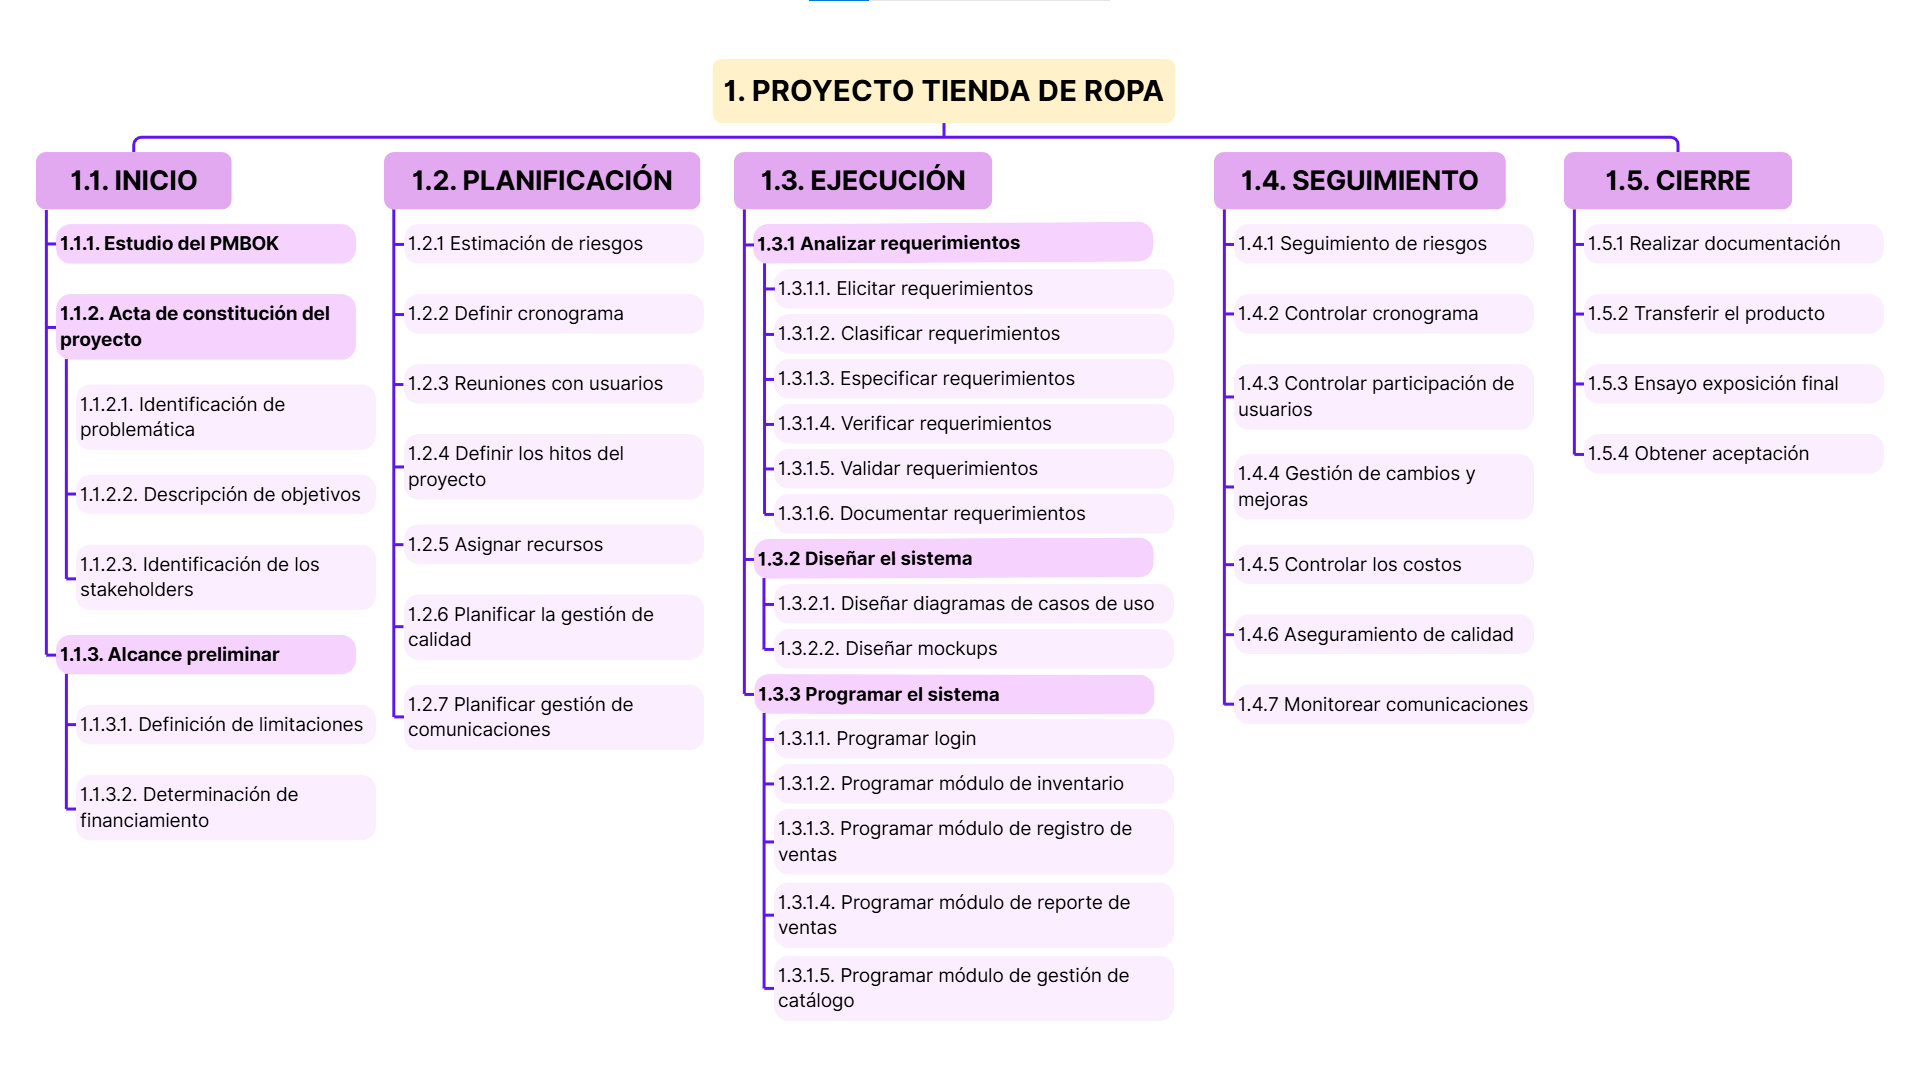
\includegraphics[width=0.92\linewidth]{figures/diagrama_edt.png}
\caption{Estructura de Desglose de Trabajo (EDT) del Proyecto SYSELL.}
\label{fig:anexo_edt}
\end{figure}

\begin{figure}[H]
\centering
\begin{subfigure}[b]{0.95\textwidth}
    \centering
    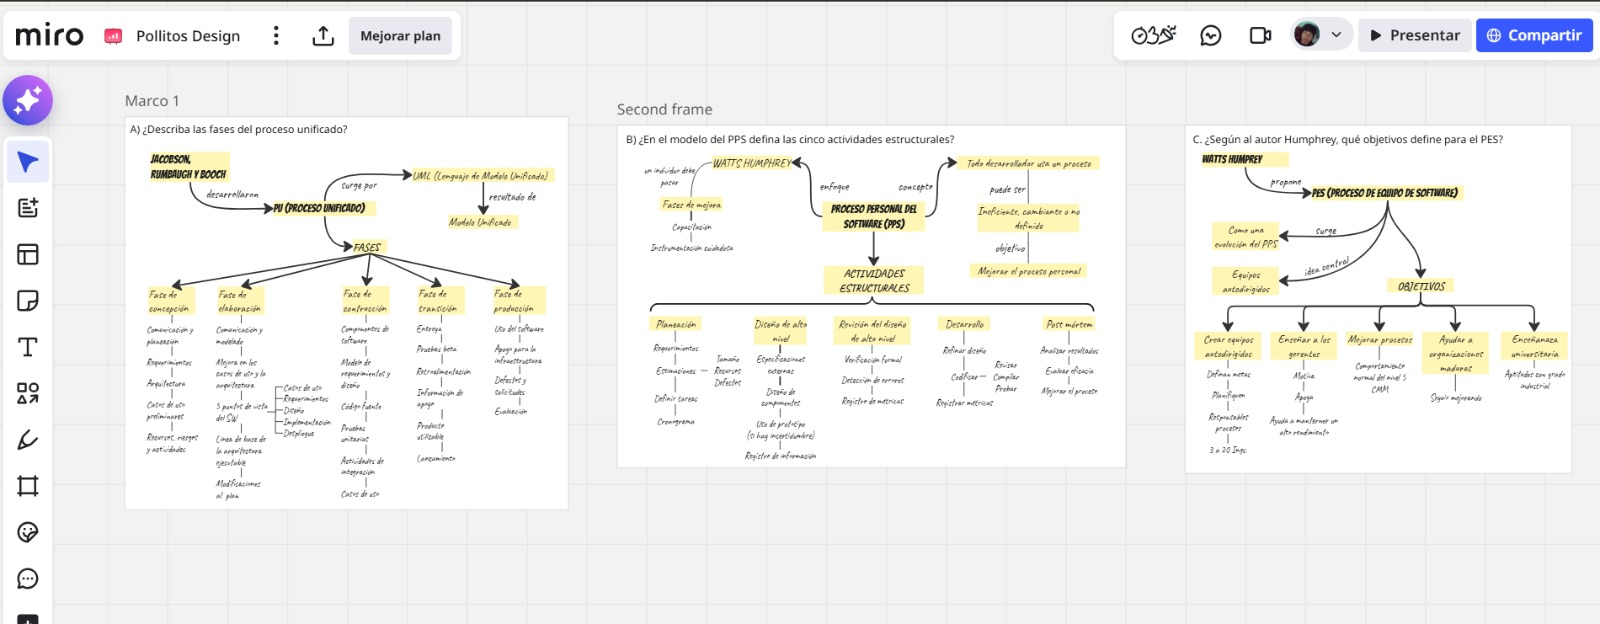
\includegraphics[width=\textwidth]{figures/miro_taskboard_1.png}
    \caption{TaskBoard en Miro --- Vista General del Backlog y Sprints de Desarrollo.}
    \label{fig:miro_1}
\end{subfigure}
\par\vspace{0.4cm}
\begin{subfigure}[b]{0.48\textwidth}
    \centering
    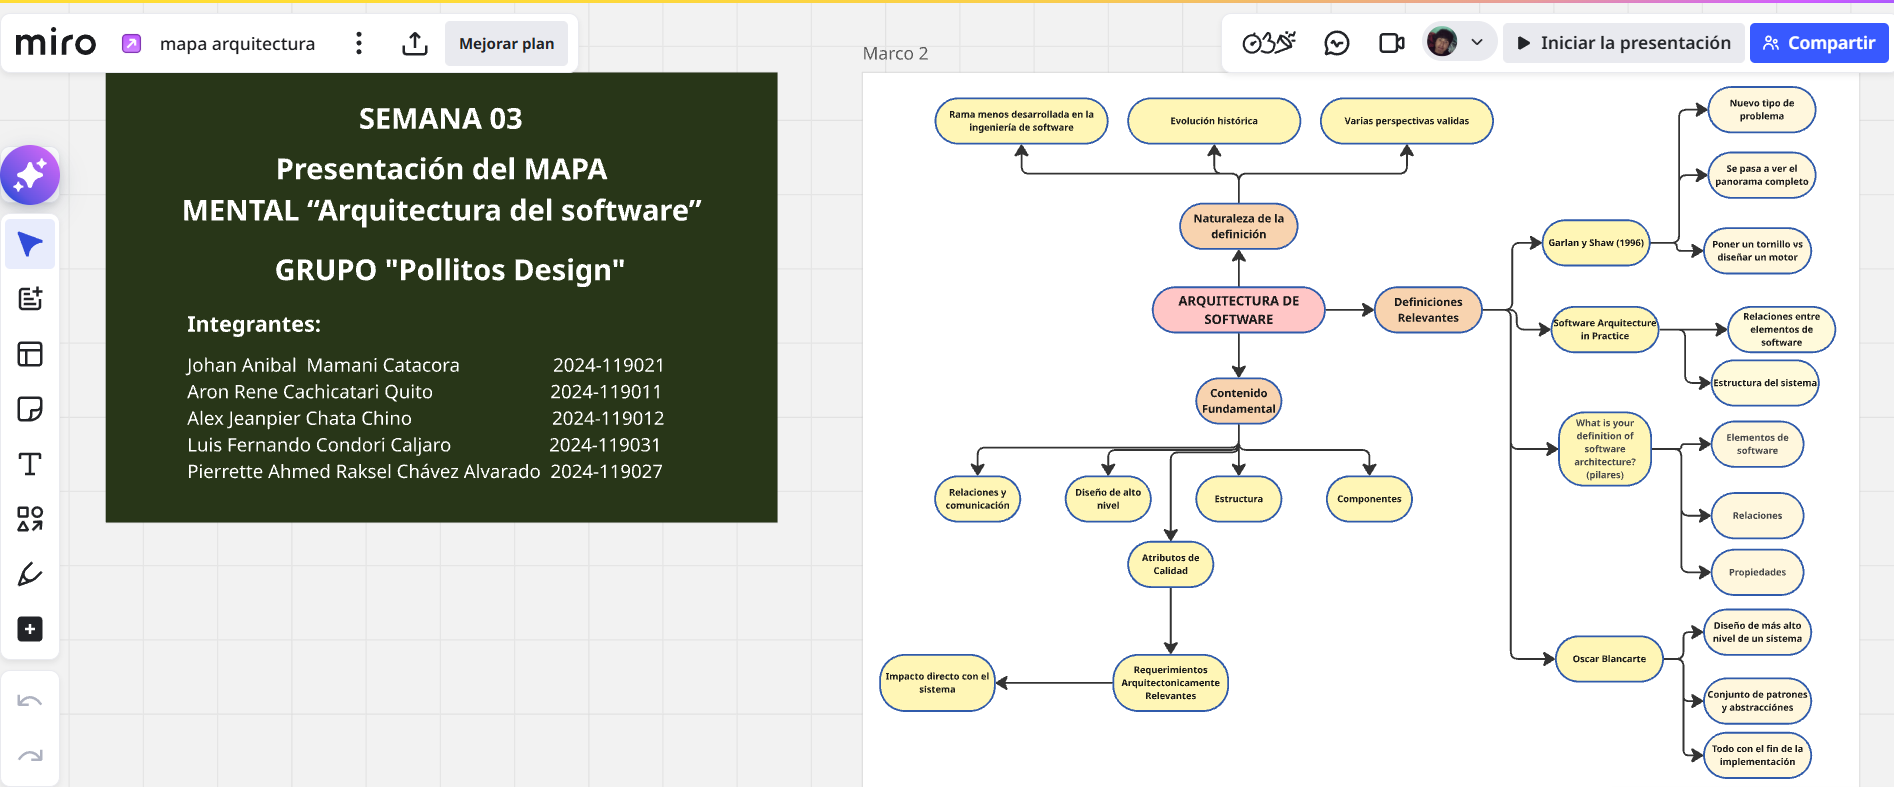
\includegraphics[width=\textwidth]{figures/miro_taskboard_2.png}
    \caption{Flujo de Tareas en Progreso y Testing.}
    \label{fig:miro_2}
\end{subfigure}
\hfill
\begin{subfigure}[b]{0.48\textwidth}
    \centering
    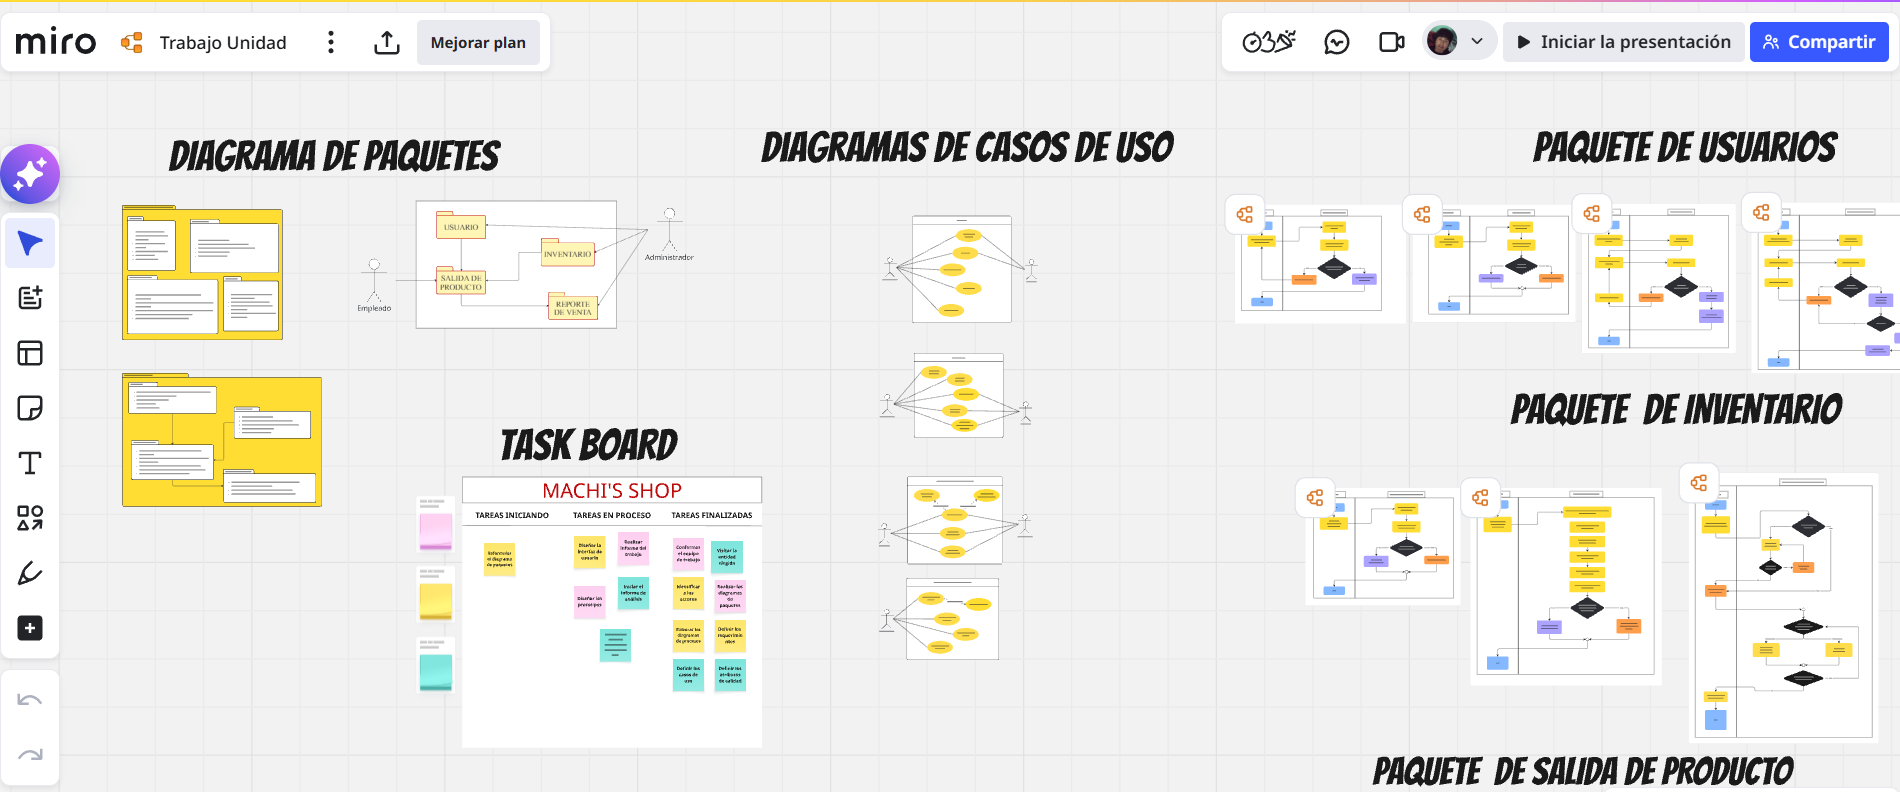
\includegraphics[width=\textwidth]{figures/miro_taskboard_3.png}
    \caption{Definición de Criterios de Aceptación (Done).}
    \label{fig:miro_3}
\end{subfigure}
\caption{Evidencias de Gestión Ágil y TaskBoard en Miro.}
\label{fig:anexo_miro}
\end{figure}

\subsection{Anexo B: Informes de Auditoría de Calidad (Interna y Externa)}

Durante el ciclo de desarrollo se llevaron a cabo evaluaciones formales de auditoría para asegurar el cumplimiento de los estándares de arquitectura y la norma ISO/IEC 25010:

\begin{figure}[H]
\centering
\begin{subfigure}[b]{0.31\textwidth}
    \centering
    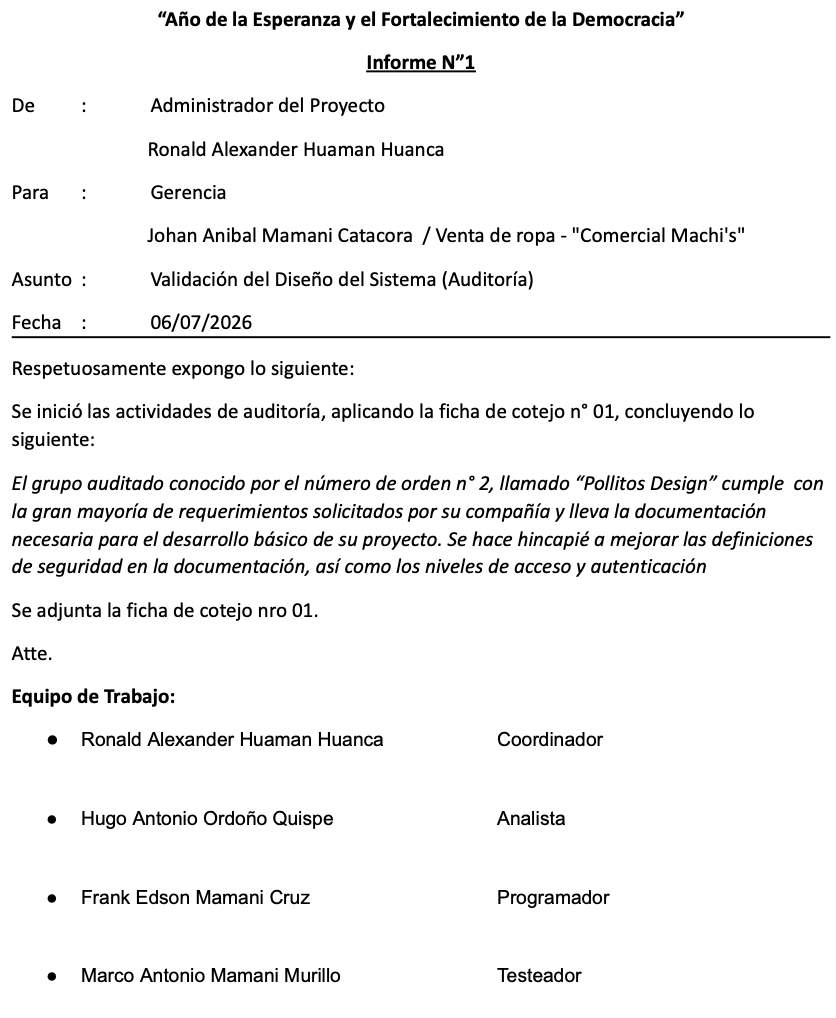
\includegraphics[width=\textwidth]{figures/auditoria_interna_p1.png}
    \caption{Auditoría Interna (Pág. 1).}
\end{subfigure}
\hfill
\begin{subfigure}[b]{0.31\textwidth}
    \centering
    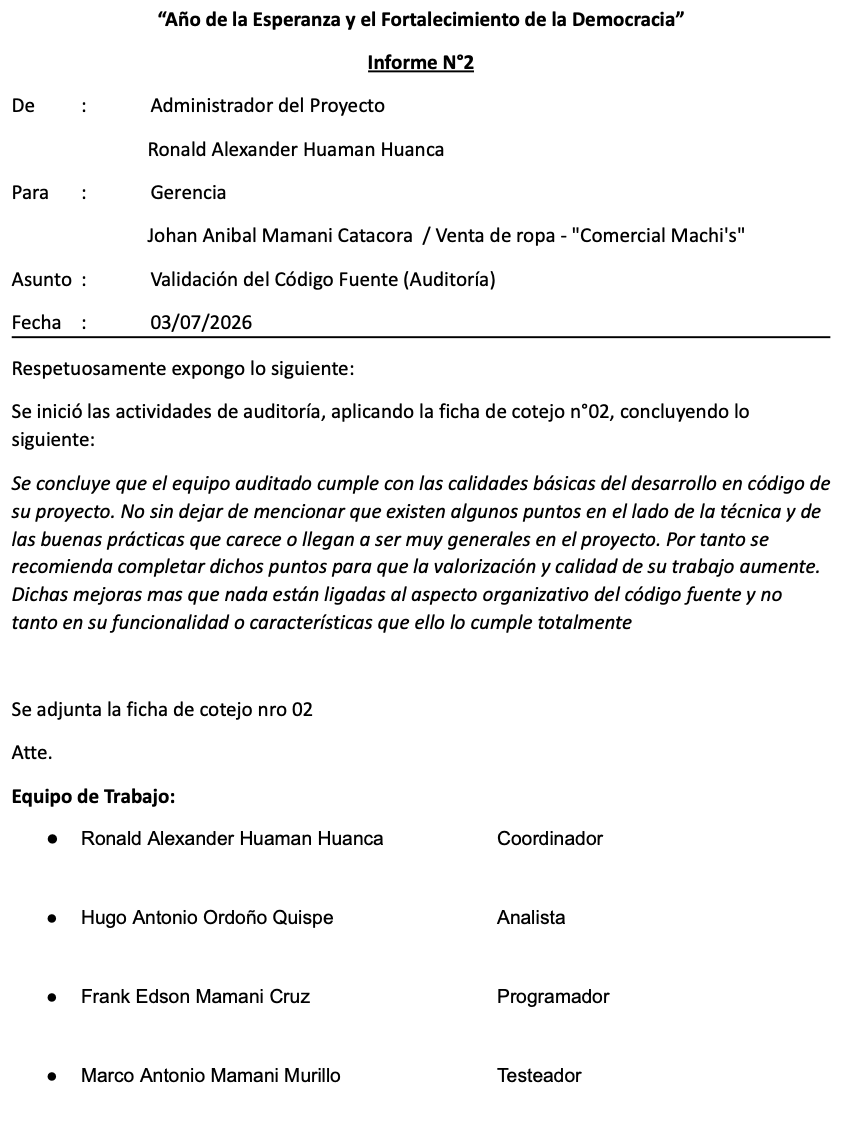
\includegraphics[width=\textwidth]{figures/auditoria_interna_p2.png}
    \caption{Auditoría Interna (Pág. 2).}
\end{subfigure}
\hfill
\begin{subfigure}[b]{0.31\textwidth}
    \centering
    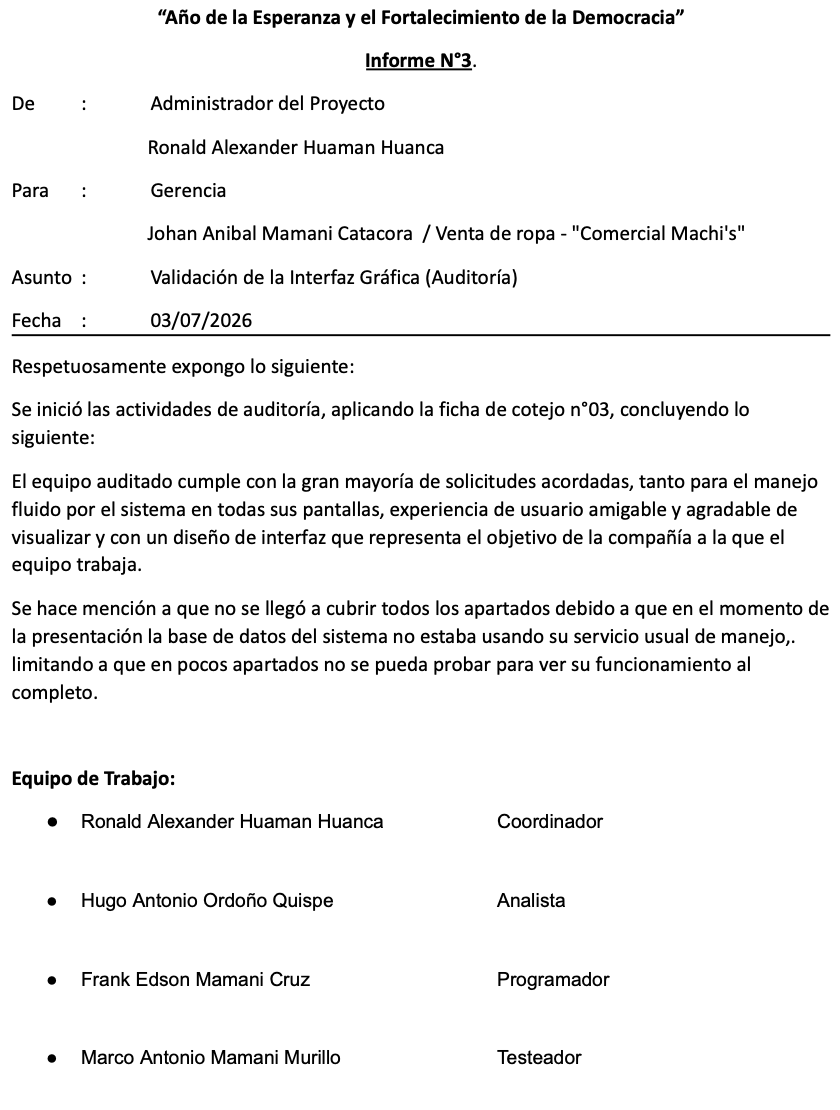
\includegraphics[width=\textwidth]{figures/auditoria_interna_p3.png}
    \caption{Auditoría Interna (Pág. 3).}
\end{subfigure}
\caption{Actas e Informes de Auditoría Interna de Software.}
\label{fig:anexo_auditoria_interna}
\end{figure}

\begin{figure}[H]
\centering
\begin{subfigure}[b]{0.48\textwidth}
    \centering
    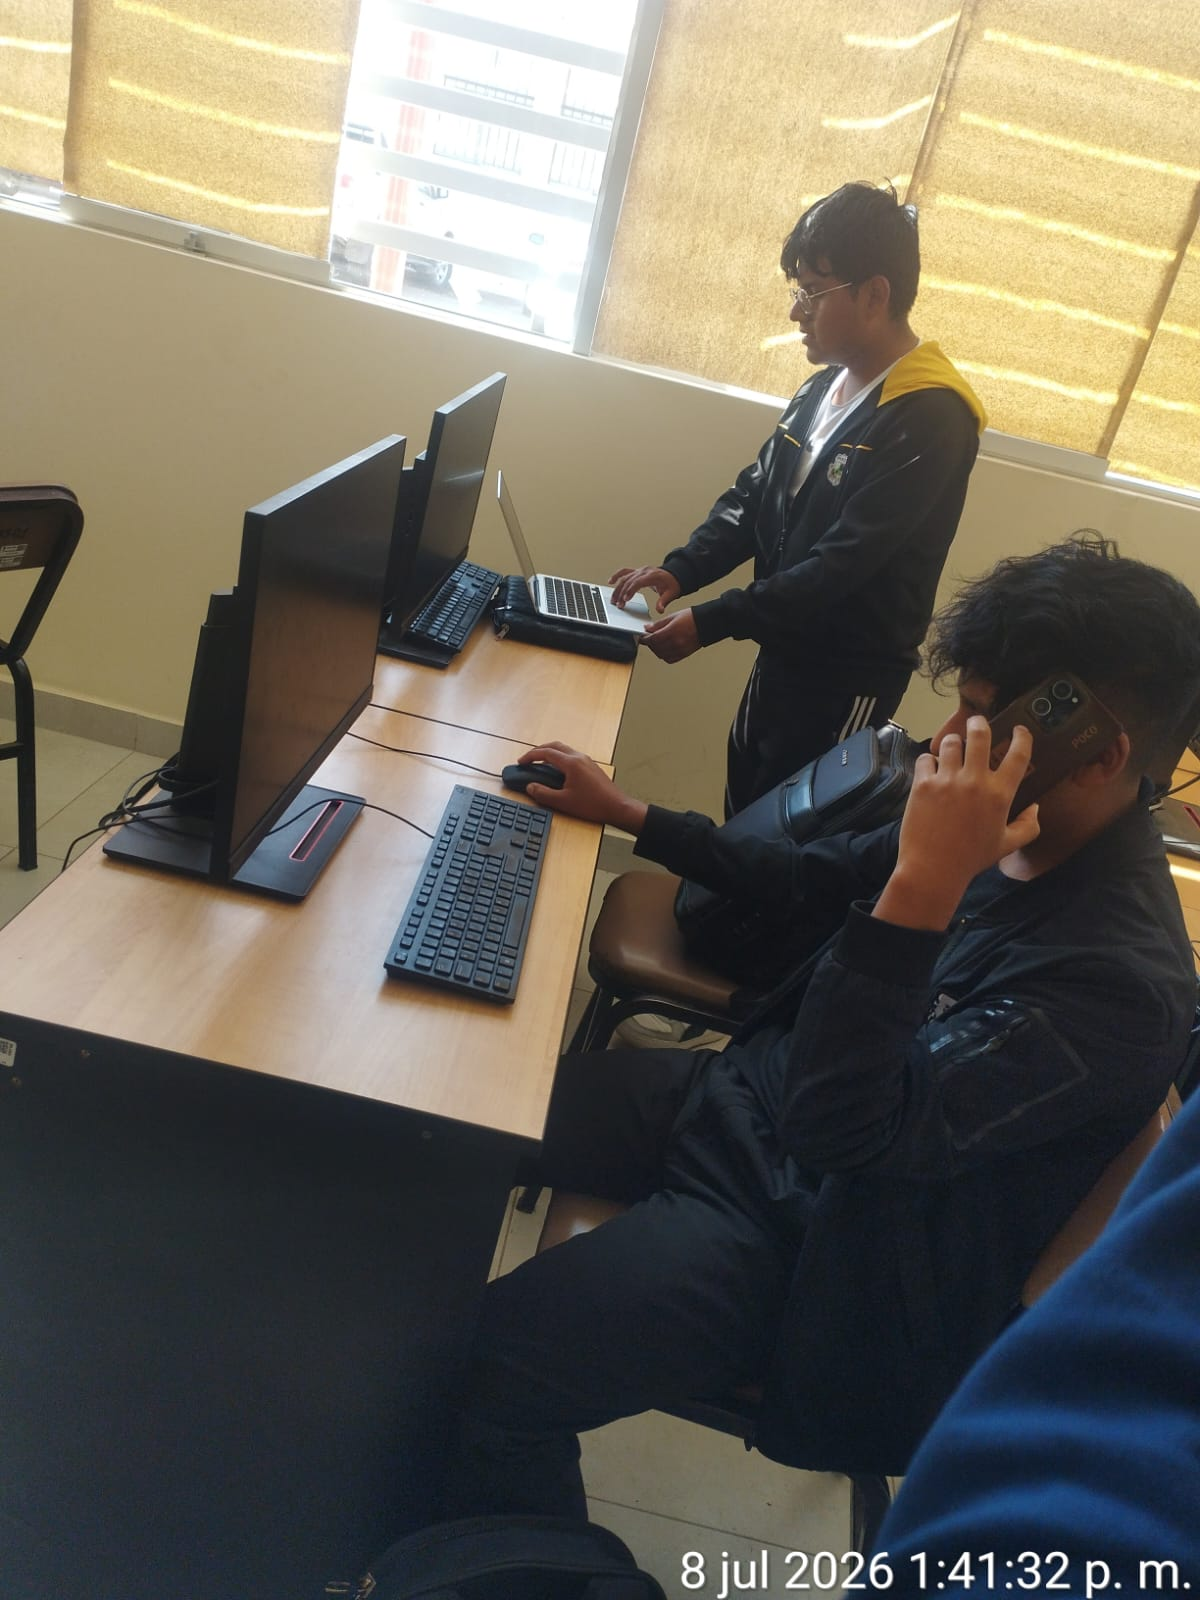
\includegraphics[width=\textwidth]{figures/auditoria_externa_p1.png}
    \caption{Informe de Auditoría Externa N° 3 --- Hallazgos.}
\end{subfigure}
\hfill
\begin{subfigure}[b]{0.48\textwidth}
    \centering
    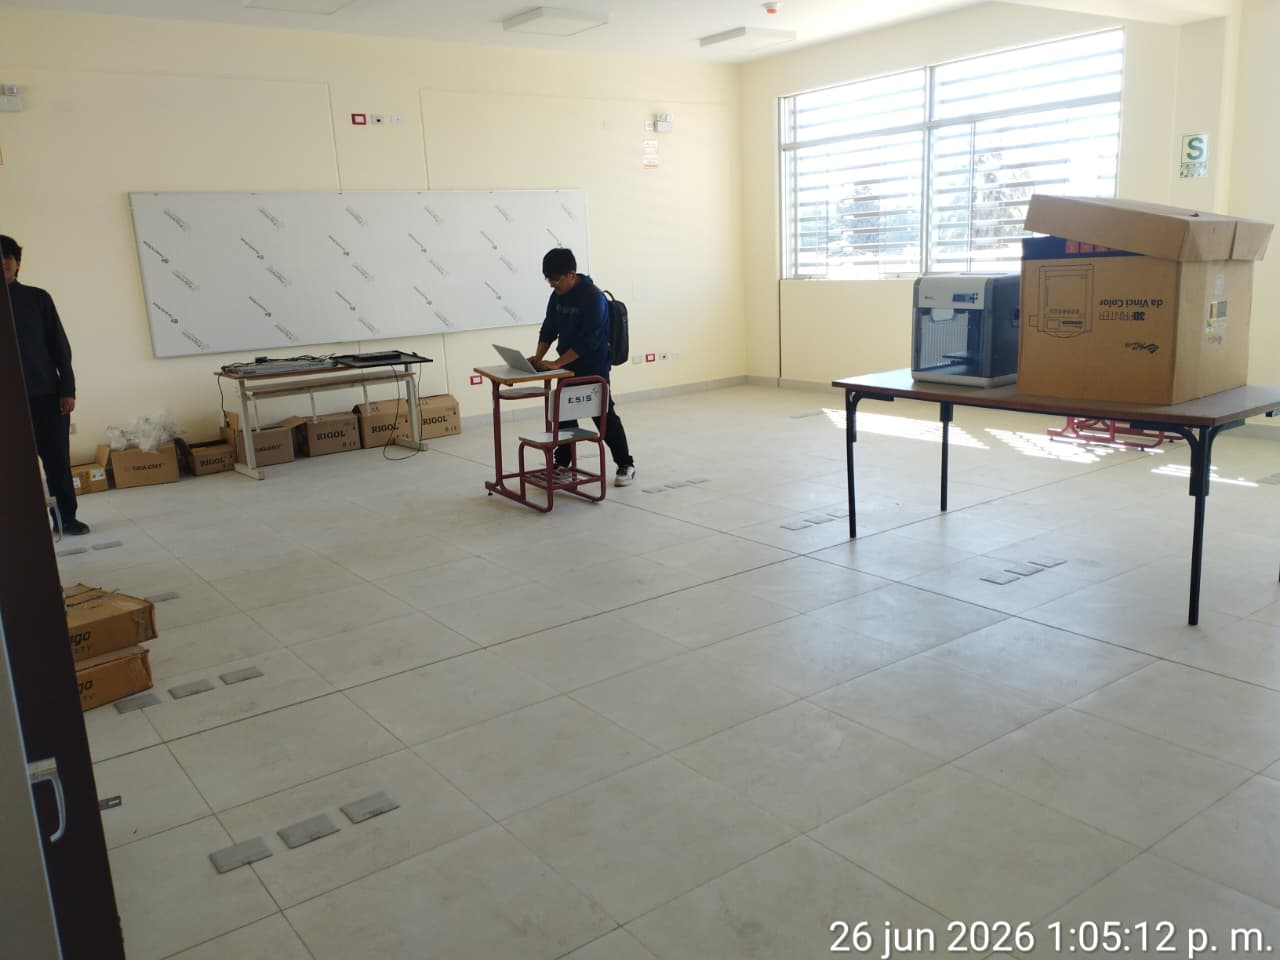
\includegraphics[width=\textwidth]{figures/auditoria_externa_p2.png}
    \caption{Conclusiones y Acciones Correctivas de Auditoría Externa.}
\end{subfigure}
\caption{Dictámenes de Auditoría Externa del Sistema SYSELL.}
\label{fig:anexo_auditoria_externa}
\end{figure}

\subsection{Anexo C: Evidencias de Trabajo de Campo y Equipo}

\begin{figure}[H]
\centering
\begin{subfigure}[b]{0.48\textwidth}
    \centering
    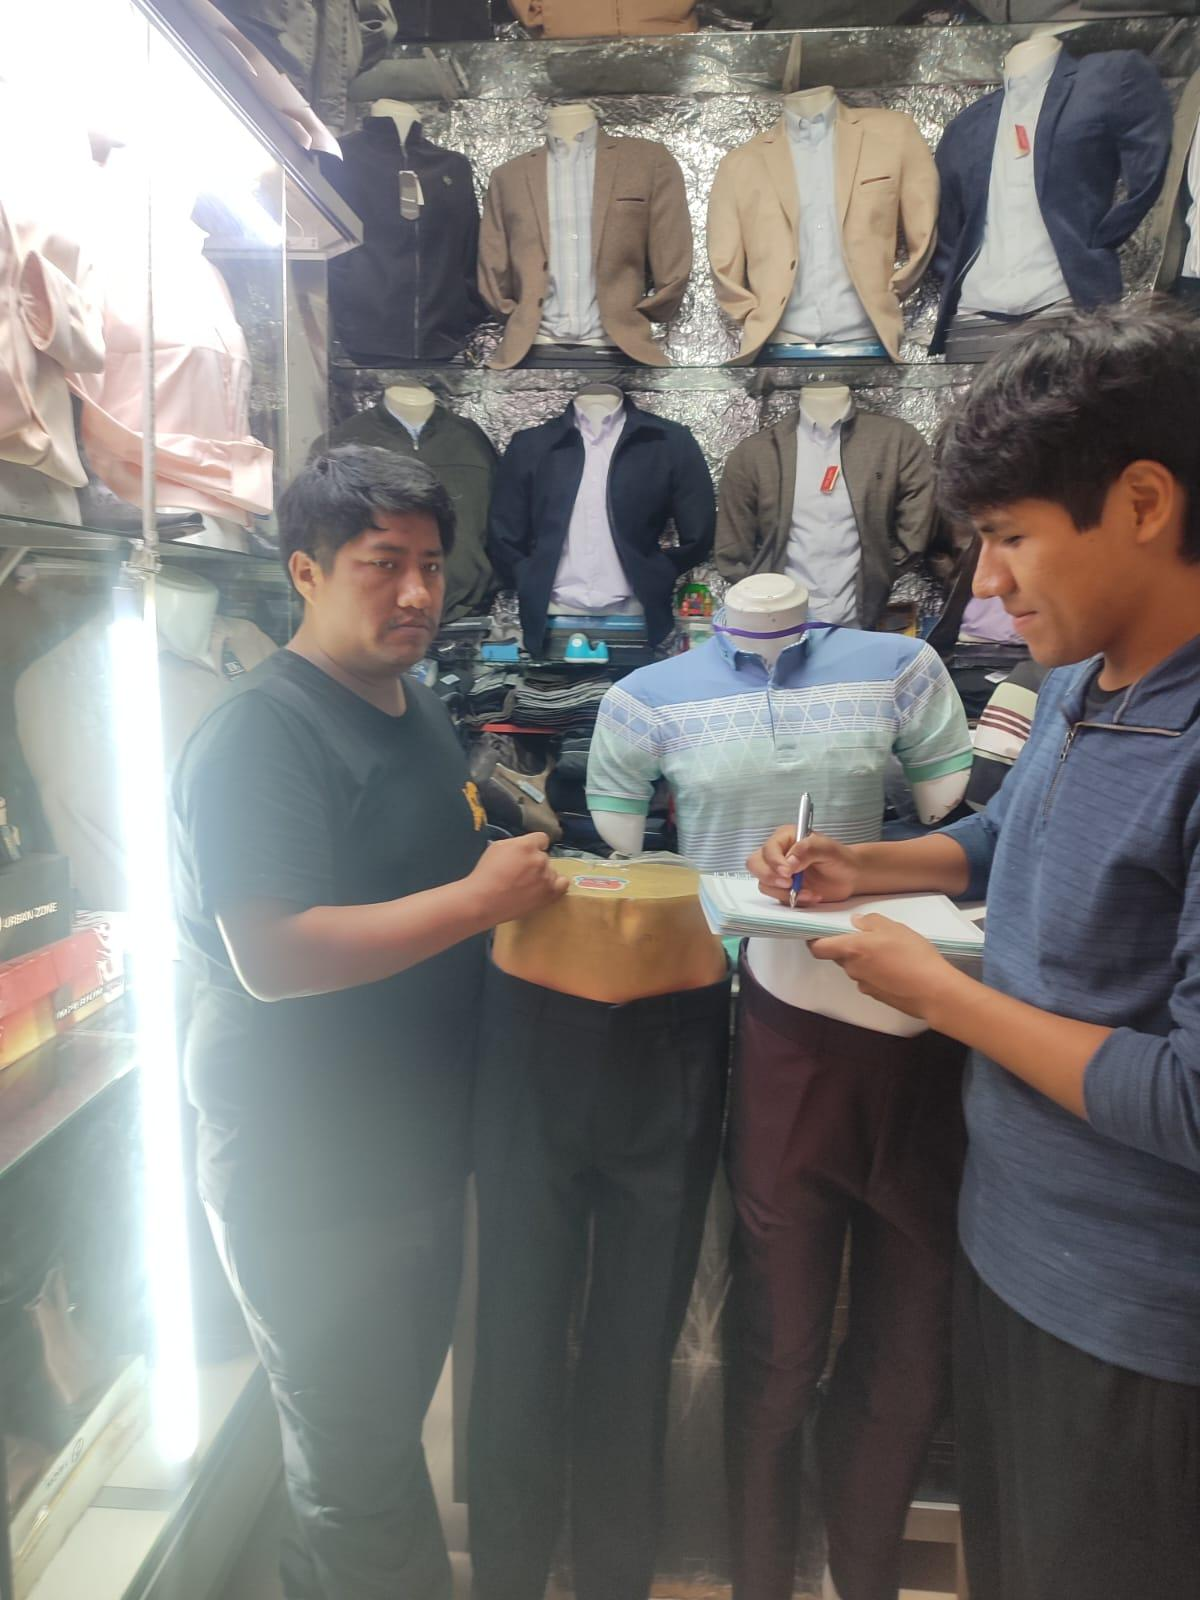
\includegraphics[width=\textwidth]{figures/evidencia_visita_tienda.jpg}
    \caption{Visita Técnica a Comercial Machi's (Levantamiento de Información).}
    \label{fig:visita_tienda}
\end{subfigure}
\hfill
\begin{subfigure}[b]{0.48\textwidth}
    \centering
    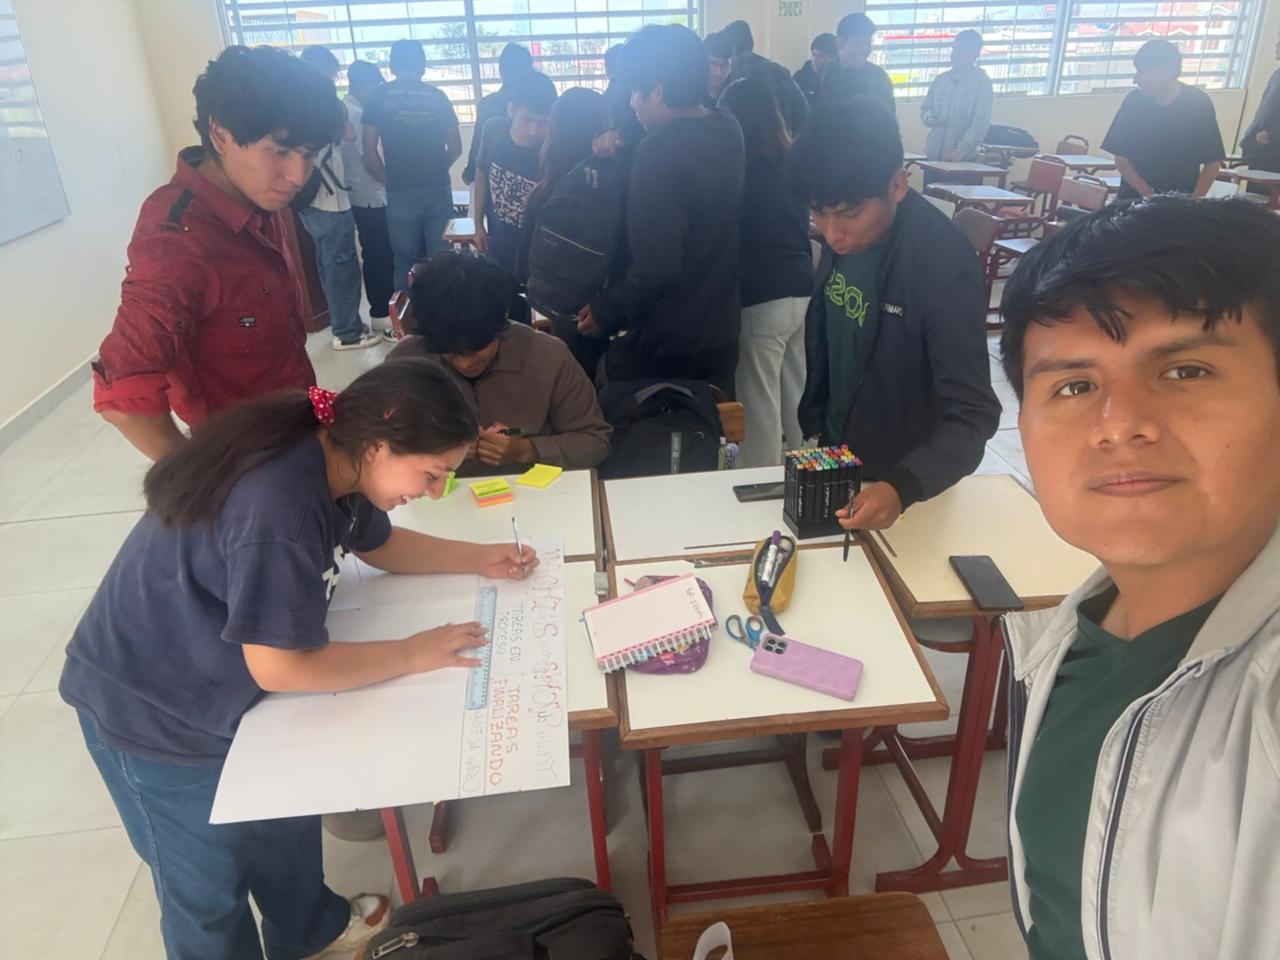
\includegraphics[width=\textwidth]{figures/evidencia_equipo_1.png}
    \caption{Sesión de Trabajo y Modelado de Arquitectura.}
    \label{fig:equipo_1}
\end{subfigure}
\par\vspace{0.4cm}
\begin{subfigure}[b]{0.48\textwidth}
    \centering
    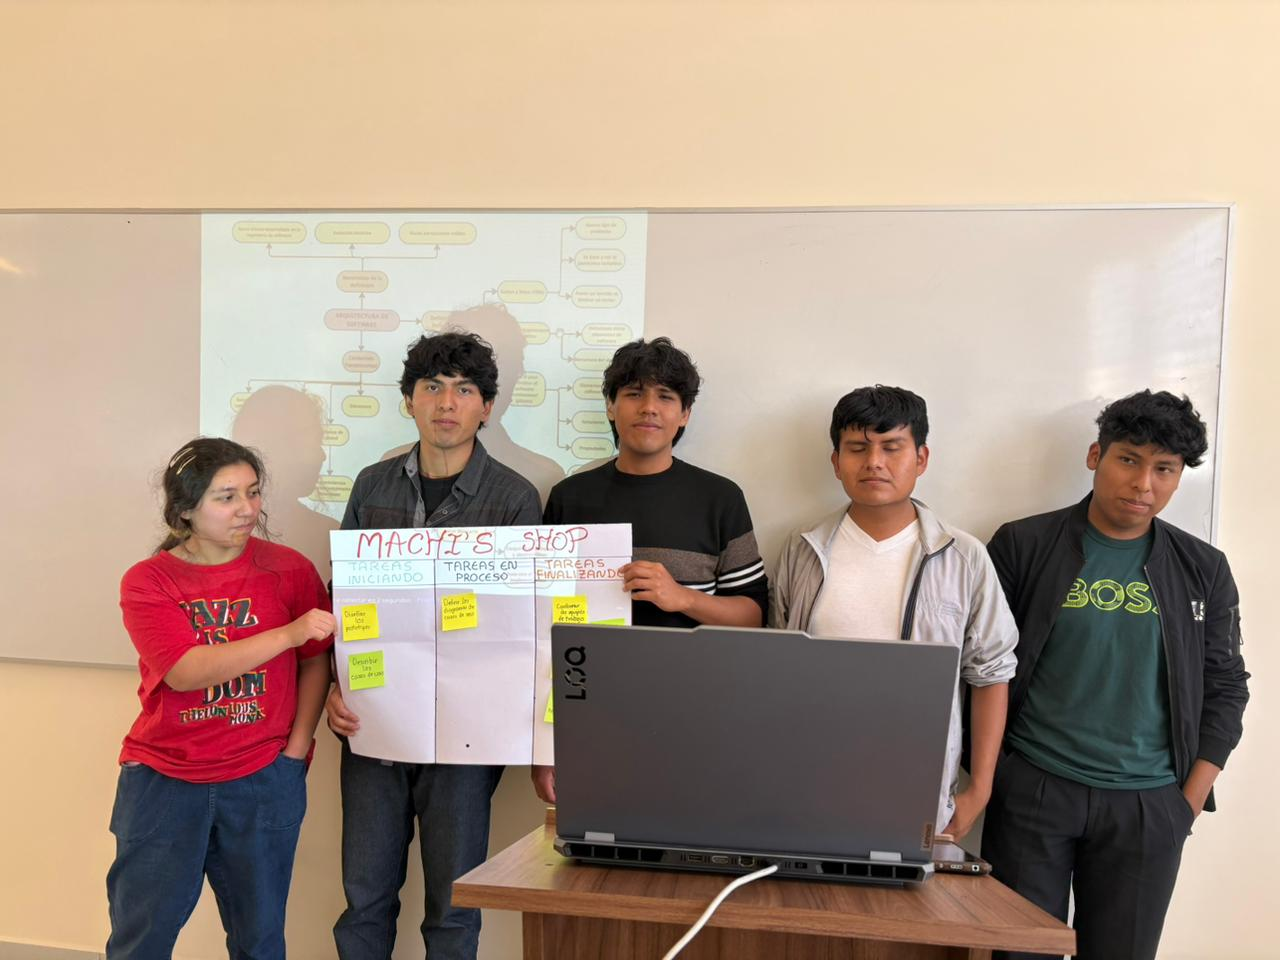
\includegraphics[width=\textwidth]{figures/evidencia_equipo_2.png}
    \caption{Revisión de Casos de Uso y Base de Datos.}
    \label{fig:equipo_2}
\end{subfigure}
\hfill
\begin{subfigure}[b]{0.48\textwidth}
    \centering
    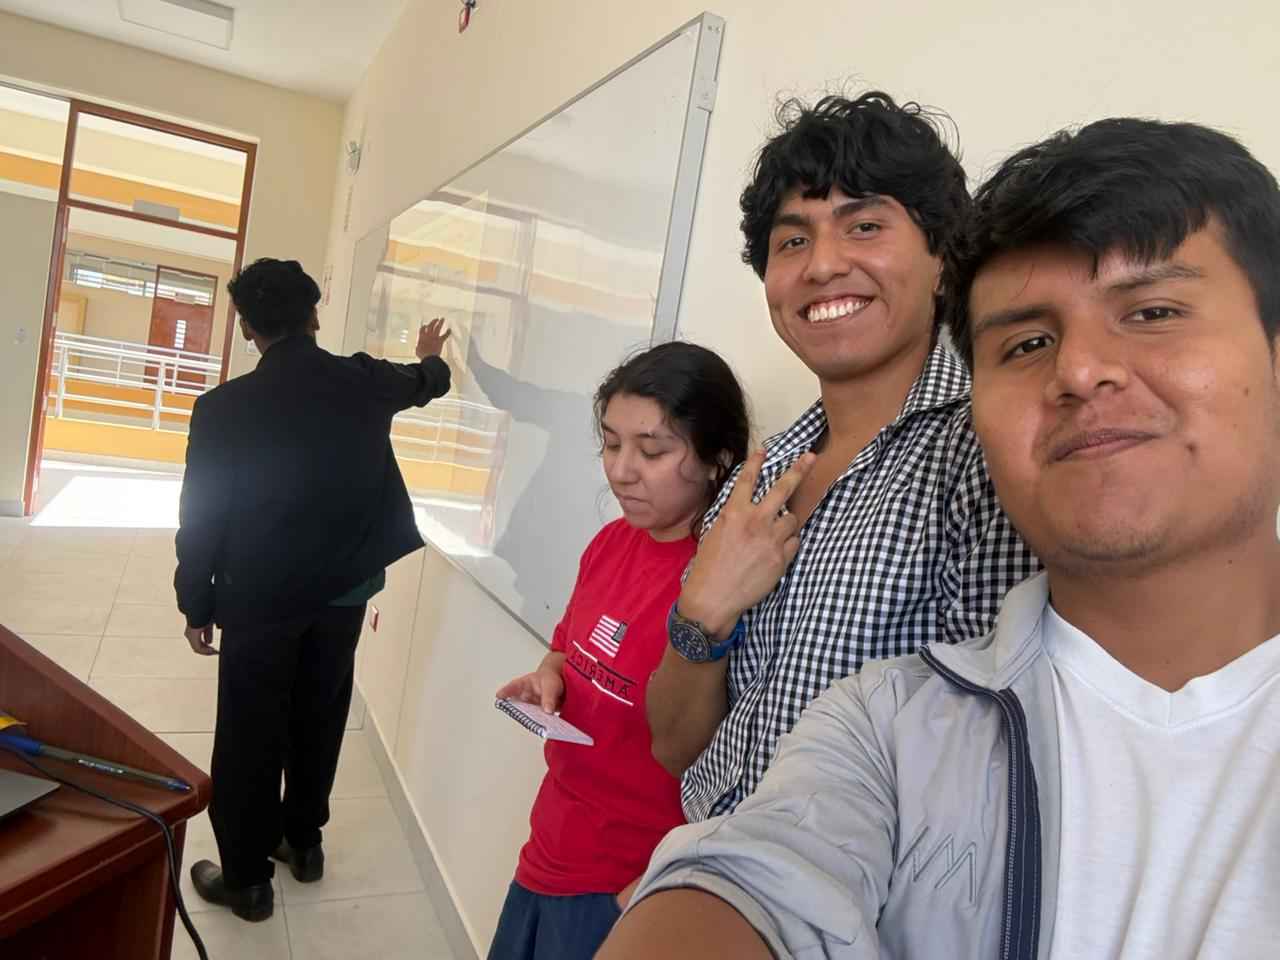
\includegraphics[width=\textwidth]{figures/evidencia_equipo_3.png}
    \caption{Sesión de Validación y Pruebas con el Asesor.}
    \label{fig:equipo_3}
\end{subfigure}
\caption{Evidencias Fotográficas del Equipo de Desarrollo y Visitas Técnicas.}
\label{fig:anexo_fotos_equipo}
\end{figure}

\subsection{Anexo D: Matriz de Trazabilidad de Requisitos (RTM)}

A continuación se resume la matriz de trazabilidad entre Requerimientos Funcionales, Reglas de Negocio, Historias de Usuario y Métodos de la API REST del backend:

\begin{table}[H]
\centering
\scriptsize
\begin{tabularx}{\linewidth}{l>{\raggedright\arraybackslash}Xll>{\raggedright\arraybackslash}p{4.5cm}}
\toprule
\rowcolor{LightSlate}
\textbf{Req.} & \textbf{Descripción Resumida} & \textbf{Regla} & \textbf{HU} & \textbf{Endpoint API REST Backend} \\
\midrule
\textbf{R-01} & Registro de Empleados & RN-08 & HU-01 & \texttt{POST /api/v1/users} \\
\textbf{R-02} & Login y Autenticación Sanctum & RN-08 & HU-01 & \texttt{POST /api/v1/auth/login} \\
\textbf{R-04} & Baja Lógica Empleado (Soft Delete) & RN-04 & HU-07 & \texttt{DELETE /api/v1/users/\{id\}} \\
\textbf{R-06} & Salida y Descuento Atómico de Stock & RN-02 & HU-03 & \texttt{POST /api/v1/sales} \\
\textbf{R-07} & Registro de Ganancias y Margen & RN-01 & HU-03 & \texttt{GET /api/v1/metrics/profit} \\
\textbf{R-08} & Registro de Venta POS en Mostrador & RN-01 & HU-03 & \texttt{POST /api/v1/sales} \\
\textbf{R-09} & Búsqueda Rápida de Productos & RN-10 & HU-03 & \texttt{GET /api/v1/products/search} \\
\textbf{R-10} & Restricción de Ingresos a Admin & RN-09 & HU-01 & \texttt{GET /api/v1/finances} \\
\textbf{R-12} & Alerta de Stock Mínimo & RN-03 & HU-04 & \texttt{GET /api/v1/inventory/alerts} \\
\textbf{R-14} & Baja Lógica Producto (Soft Delete) & RN-04 & HU-07 & \texttt{DELETE /api/v1/products/\{id\}} \\
\textbf{R-18} & Exportación Reportes PDF/Excel & RN-01 & HU-06 & \texttt{GET /api/v1/reports/export} \\
\textbf{R-19} & Devoluciones y Cambios & RN-06 & HU-05 & \texttt{POST /api/v1/returns} \\
\textbf{R-20} & Gestión de Múltiples Locales & RN-02 & HU-06 & \texttt{POST /api/v1/stores} \\
\textbf{R-23} & Cierre Diario de Caja y Arqueo & RN-07 & HU-06 & \texttt{POST /api/v1/cash/close} \\
\textbf{R-24} & Recuperación de Contraseña & RN-08 & HU-01 & \texttt{POST /api/v1/auth/forgot-password} \\
\textbf{R-25} & Bloqueo y Cierre Inactividad & RN-08 & HU-02 & \textit{Middleware / Sanctum} \\
\textbf{R-26} & Logs de Auditoría del Sistema & RN-09 & HU-07 & \texttt{GET /api/v1/audit-logs} \\
\textbf{R-27} & Filtros Multicriterio (Talla/Color) & RN-10 & HU-03 & \texttt{GET /api/v1/products/filter} \\
\textbf{R-28} & Dashboard Ejecutivo Tiempo Real & RN-01 & HU-01 & \texttt{GET /api/v1/dashboard/kpis} \\
\bottomrule
\end{tabularx}
\caption{Matriz de Trazabilidad de Requisitos (RTM) del Sistema SYSELL.}
\label{tab:matriz_trazabilidad}
\end{table}
